\section{ATAN2 Inverse Trigonometric 4-Quadrant Arctangent Function}

\subsection{Usage}

Computes the \verb|atan2| function for its argument.  The general
syntax for its use is
\begin{verbatim}
  z = atan2(y,x)
\end{verbatim}
where \verb|x| and \verb|y| are \verb|n|-dimensional arrays of numerical type.
Integer types are promoted to the \verb|double| type prior to
calculation of the \verb|atan2| function. The size of the output depends
on the size of \verb|x| and \verb|y|.  If \verb|x| is a scalar, then \verb|z|
is the same size as \verb|y|, and if \verb|y| is a scalar, then \verb|z|
is the same size as \verb|x|.  The type of the output is equal to the type of
|y/x|.  
\subsection{Function Internals}

The function is defined (for real values) to return an 
angle between \verb|-pi| and \verb|pi|.  The signs of \verb|x| and \verb|y|
are used to find the correct quadrant for the solution.  For complex
arguments, the two-argument arctangent is computed via
\[
  \mathrm{atan2}(y,x) \equiv -i \log\left(\frac{x+i y}{\sqrt{x^2+y^2}} \right)
\]
For real valued arguments \verb|x,y|, the function is computed directly using 
the standard C library's numerical \verb|atan2| function. For both 
real and complex arguments \verb|x|, note that generally
\[
  \mathrm{atan2}(\sin(x),\cos(x)) \neq x,
\]
due to the periodicities of  \verb|cos(x)| and \verb|sin(x)|.
\subsection{Example}

The following code demonstates the difference between the \verb|atan2| 
function and the \verb|atan| function over the range \verb|[-pi,pi]|.
\begin{verbatim}
--> x = linspace(-pi,pi);
--> sx = sin(x); cx = cos(x);
--> plot(x,atan(sx./cx),x,atan2(sx,cx))
\end{verbatim}


\centerline{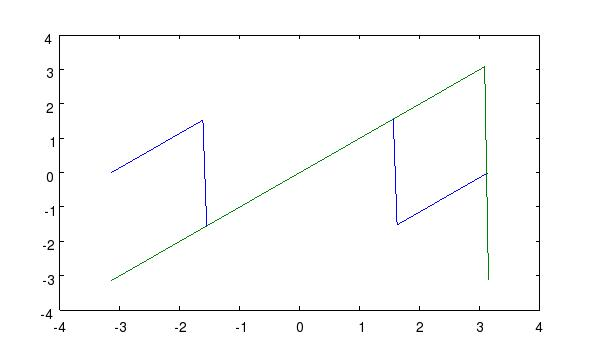
\includegraphics[width=8cm]{atan2plot}}

Note how the two-argument \verb|atan2| function (green line) 
correctly ``unwraps'' the phase of the angle, while the \verb|atan| 
function (red line) wraps the angle to the interval \verb|[-i/2,i/2]|.
